% =====================================================================
%  ISDS 2026 -- The 4th International Conference on Intelligent Systems
%  and Data Science, Yuan Ze University, Taiwan, 14-15 November 2026
%
%  COMPACT long-paper variant, trimmed to the 12-15 page limit.
%  Format: Springer LNCS/CCIS one-column (llncs.cls), English, PDF.
%  Track 3 -- Image Processing & Pattern Recognition
%  Submission: https://easychair.org/conferences/?conf=isds2026
%
%  Trimmed relative to ISDS2026_FGSS.tex (see ISDS2026_SUBMISSION_CHECK.md):
%    - 12 figures -> 5   (kept: architecture, qualitative grid, frequency
%      decomposition, robustness overview, training curve)
%    - 11 tables  -> 6   (dropped: relwork positioning, loss cheat-sheet,
%      cross-family SOTA context, inference budget -> moved to prose;
%      serial-2 and serial-3 merged into one table, blend_* rows dropped;
%      ablation table also folded into prose to meet the 12-15 page limit)
%    - Introduction 6 -> 3 paragraphs; reverse-decoder / reverse-loss and
%      protocol / implementation subsections condensed; loss hyper-parameter
%      list moved to a footnote
%  Build: pdflatex ISDS2026_FGSS_compact (x2)
% =====================================================================
\documentclass[conference]{IEEEtran}
\IEEEoverridecommandlockouts

\usepackage{cmap}
\usepackage[T1]{fontenc}
\usepackage[utf8]{inputenc}
\usepackage{amsmath,amssymb,amsfonts}
\usepackage{graphicx}
\usepackage{textcomp}
\usepackage[table]{xcolor}
\usepackage{booktabs}
\usepackage{multirow}
\usepackage{array}
\usepackage{url}
\usepackage{float}
\usepackage{colortbl}
\usepackage{algorithm}
\usepackage{algpseudocode}

\usepackage[hidelinks]{hyperref}
\providecommand{\doi}[1]{\href{https://doi.org/#1}{https://doi.org/#1}}

\renewcommand{\arraystretch}{1.0}
\setlength{\tabcolsep}{4pt}
\definecolor{rowshade}{HTML}{F2F2F2}

\setlength{\textfloatsep}{8pt plus 1.0pt minus 2.0pt}
\setlength{\floatsep}{6pt plus 1.0pt minus 2.0pt}
\setlength{\intextsep}{8pt plus 1.0pt minus 2.0pt}
\setlength{\abovecaptionskip}{3pt}
\setlength{\belowcaptionskip}{-3pt}

\begin{document}

\title{Frequency-Guided Semantic Steganography for High-Fidelity Self-Contained Style-Transfer Image Hiding}

\author{
\IEEEauthorblockN{Ngoc-Giau Pham}
\IEEEauthorblockA{\textit{Tra Vinh University}\\
Vinh Long, Vietnam\\
\textit{Tien Giang University}\\
Dong Thap, Vietnam}
\and
\IEEEauthorblockN{Phuoc-Hung Vo\thanks{Corresponding author: Phuoc-Hung Vo (e-mail: hung.vp@tvu.edu.vn).}}
\IEEEauthorblockA{\textit{Tra Vinh University}\\
Vinh Long, Vietnam\\
hung.vp@tvu.edu.vn}
\and
\IEEEauthorblockN{Hong-Ngoc Tran}
\IEEEauthorblockA{\textit{Vietnamese-German University}\\
Ho Chi Minh City, Vietnam}
}

\maketitle

\begin{abstract}
% SOURCE: run_summary.json, paper_table_main.csv, token_summary.csv, ablation.csv, robustness_metrics.csv
Style transfer steganography conceals data within artistic brushstrokes, but methods in this family typically report cover PSNR in the $33$--$36$\,dB range and fail under repeated re-stylisation. These limitations often stem from unbounded capacity penalties that leak embedding energy into low-frequency structures, alongside spatial payload representations that strain the carrier's capacity. To overcome these issues, we propose a frequency-guided semantic steganography network (FGSS). We first compress the secret into a compact $64\!\times\!32\!\times\!32$ semantic token and a thumbnail, reducing bandwidth requirements by roughly a factor of three. We then introduce a nonlinear capacity ceiling that maps a target PSNR to a soft barrier on the cover MSE. To further hide the residual, a frequency loss inspired by the discrete wavelet transform confines the perturbations to the high-frequency band. Finally, we employ an oracle-guided reverse decoder and a probabilistic future pass so that the self-contained stylisation survives up to two further re-stylisations, i.e. three cumulative stylisation passes. Evaluated on $600$ pairs from COCO\,val2017 across five painting styles, FGSS achieves $39.61\pm0.35$\,dB cover PSNR and $0.9914$ SSIM. It improves reverse SSIM from $0.52$ (naive baseline) to $0.81$, and maintains token stability under JPEG and Gaussian noise. Ablation studies confirm the capacity ceiling alone provides a $5.76$\,dB gain. Cross-dataset tests demonstrate consistent $\approx\!40$\,dB PSNR, and robustness checks across $11$ attacks show negligible token drift. The embedding path needs only $1.9$\,M of the system's $10.7$\,M parameters and embeds a $256\!\times\!256$ image in under $0.01$\,s on a consumer GPU.
\end{abstract}

\begin{IEEEkeywords}
Image steganography, Neural style transfer, Frequency-domain learning, Capacity ceiling, Robustness, Semantic tokens.
\end{IEEEkeywords}

\section{Introduction}

Hiding information inside ordinary-looking images is a fundamental technique in digital communication. Deep learning has substantially extended the achievable payload capacity relative to LSB-based predecessors; however, the residuals introduced by deep encoders exhibit statistical fingerprints that contemporary steganalysers detect with considerable accuracy~\cite{isn,riis}. One countermeasure is to alter the statistical properties of the carrier itself: when the cover is a painting rather than a photograph, brush strokes and palette quantisation already introduce noise within which small additive perturbations remain visually plausible. This motivates \emph{style-transfer steganography}~\cite{wacv2020,ihst2024,sddpm2025}, and in particular its most demanding variant, \emph{self-contained} stylisation~\cite{wacv2020}, in which the stego image alone must carry sufficient information for the receiver to reconstruct the original content by inverting the stylisation process. In practice, balancing these objectives is difficult. Increasing embedding strength improves secret recoverability but introduces visible texture jitter and palette drift; reducing it preserves the cover but degrades reverse extraction; and a second or third style transfer applied to the stego image --- serial stylisation --- typically destroys most of the embedded information~\cite{wacv2020}. Consequently, most reported systems occupy a narrow region of this trade-off space, with cover-referenced PSNR typically in the $33$--$36$\,dB range, reverse SSIM below $0.6$, and serial recovery degrading rapidly beyond the second stylisation step.

This trade-off is driven by two common design choices. First, models typically use an unbounded payload capacity loss: the encoder is encouraged to keep the residual small only through a quadratic prior, which imposes no upper bound, so nothing prevents the optimiser from placing a successful solution in the low-frequency, structurally salient component of the carrier, to which the human visual system is most sensitive. Second, they rely on a spatial payload representation: secret images, dense bit grids and feature maps occupy approximately as many spatial positions as the cover itself, forcing the encoder to distribute its perturbation broadly and leaving little capacity for the carrier to absorb a subsequent stylisation pass. This work addresses both limitations. Instead of a spatial payload, the secret is distilled into a compact semantic token $\mathbf{z}\!\in\!\mathbb{R}^{64\times32\times32}$ together with a low-resolution thumbnail $\mathbf{T}$, both produced by a small CNN tokenizer. Rather than an unbounded prior, the residual is bounded by a nonlinear capacity ceiling: a quadratic penalty that activates only above an explicit threshold $\epsilon$ tied directly to a target cover PSNR. A frequency loss based on the discrete wavelet transform further constrains the spectral allocation of the residual, penalising the low band aggressively and leaving the high band unconstrained, thereby directing the perturbation into texture rather than into structure. Three further mechanisms support the system: an oracle-guided reverse loss, a serial consistency term for robustness to further re-stylisation, and a bandwise embedding allocation loss.

% SOURCE: run_summary.json (cover_metrics_mean), token_summary.csv, ablation.csv
Despite these additions the deployment cost stays low: of the $10.7$\,M trainable parameters in the full system, only the $1.9$\,M in the tokenizer and stego encoder are needed on the sending side, and that path embeds a $256\!\times\!256$ image in $0.0096$\,s on a consumer GPU. On the COCO~val2017~\cite{coco} protocol with $600$ content--style pairs and five painting references, the model achieves a cover PSNR of $39.61\pm0.35$\,dB, an SSIM~\cite{ssim} of $0.9914\pm0.0030$ and an LPIPS~\cite{lpips} of $0.0195\pm0.0081$, while the token MSE varies by at most $1\times10^{-4}$ under JPEG-style smoothing and additive Gaussian perturbations. A controlled CPU-only ablation attributes the improvement primarily to the capacity ceiling, which alone accounts for $+5.76$\,dB of cover PSNR ($35.61\to41.37$\,dB). Our contributions are: (i) a capacity ceiling formulation that maps a target cover PSNR to a soft nonlinear barrier on the cover MSE, removing the implicit fidelity/extraction trade-off; (ii) a differentiable frequency-guided loss that uses a strided average-pooling proxy of the discrete wavelet transform to confine the residual to the high-frequency band without adding learnable parameters, plus a band-localised embedding allocation loss; (iii) a semantic token payload that compresses the secret into a low-bandwidth representation so the carrier can absorb it under both constraints; (iv) an oracle-guided reverse extraction stack and a probabilistic future pass that stabilise self-contained stylisation under further re-stylisations; and (v) a controlled study on COCO with $600$ evaluation pairs covering reverse and serial recovery under three attack channels, an ablation isolating the ceiling and the frequency loss, cross-dataset generalisation on four unseen benchmarks, an $11$-attack robustness audit, GPU and CPU inference budgets, and a steganalysis evaluation with three detectors that quantifies --- rather than assumes away --- the detectability of the resulting stego images.

\section{Related Work}
\label{sec:relwork}

\subsection{Deep Image-in-Image Steganography}
The first wave of deep steganography embedded full-resolution images using encoder--decoder or generative models, introducing mechanisms like invertible networks~\cite{isn} and robust flows~\cite{riis} to balance PSNR. While effective on photorealistic carriers, small perturbations often shift statistics detectably for steganalysers like SRNet~\cite{srnet}. A second family avoids embedding entirely via semantic tokens (e.g., IDEAS~\cite{ideas2022}), offering immunity to steganalysis but severely limiting payload bandwidth. The third family, style transfer steganography, uses artistic styles to conceal embedding noise. From early self-contained stylisation~\cite{wacv2020} to recent frequency-domain~\cite{quat2021} and diffusion~\cite{sddpm2025} methods, an explicit barrier on cover distortion remains rare. Most models rely on unbounded quadratic priors. We address this gap using a capacity ceiling derived directly from a target PSNR, while combining the semantic token intuition of coverless methods with the deterministic carrier generation of style transfer.

\section{Method}
\label{sec:method}

\subsection{Notation and System Overview}
Scalars are plain math italic, vectors bold lower case, tensors bold upper case. The cover image is $\mathbf{X}_{\text{cover}}\!\in\!\mathbb{R}^{3\times H\times W}$, the secret content is $\mathbf{C}\!\in\!\mathbb{R}^{3\times H\times W}$ and the painting reference is $\mathbf{S}$. The cover is obtained by an optimisation-based stylisation operator $f_{\text{style}}(\mathbf{C},\mathbf{S})$ held fixed during stego training. We write $\mathbf{z}\!\in\!\mathbb{R}^{d_{\text{tok}}\times g_{\text{tok}}\times g_{\text{tok}}}$ for the semantic token used as payload and $\mathbf{T}\!\in\!\mathbb{R}^{3\times g_{\text{tok}}\times g_{\text{tok}}}$ for the auxiliary thumbnail, with $g_{\text{tok}}=32$ and $d_{\text{tok}}=64$ throughout; because the tokenizer ends in an adaptive pooling stage, the same token geometry is produced at both the $256\!\times\!256$ benchmark resolution and the $192\!\times\!192$ CPU resolution.

The system consists of four learnable modules --- a semantic tokenizer $f_{\text{tok}}$, a stego encoder $f_{\text{enc}}$, a stego decoder $f_{\text{dec}}$ and a reverse decoder $f_{\text{rev}}$ --- together with a non-learnable attack channel $\mathcal{A}$. All four are trained jointly; Figure~\ref{fig:architecture} summarises the data flow. Training and inference share the same flow. The channel is enumerated over its three modes in both regimes: during training so the decoder sees clean and degraded inputs in a balanced fashion, and at evaluation so every pair is scored under each mode separately.

\begin{figure}[htbp]
    \centering
    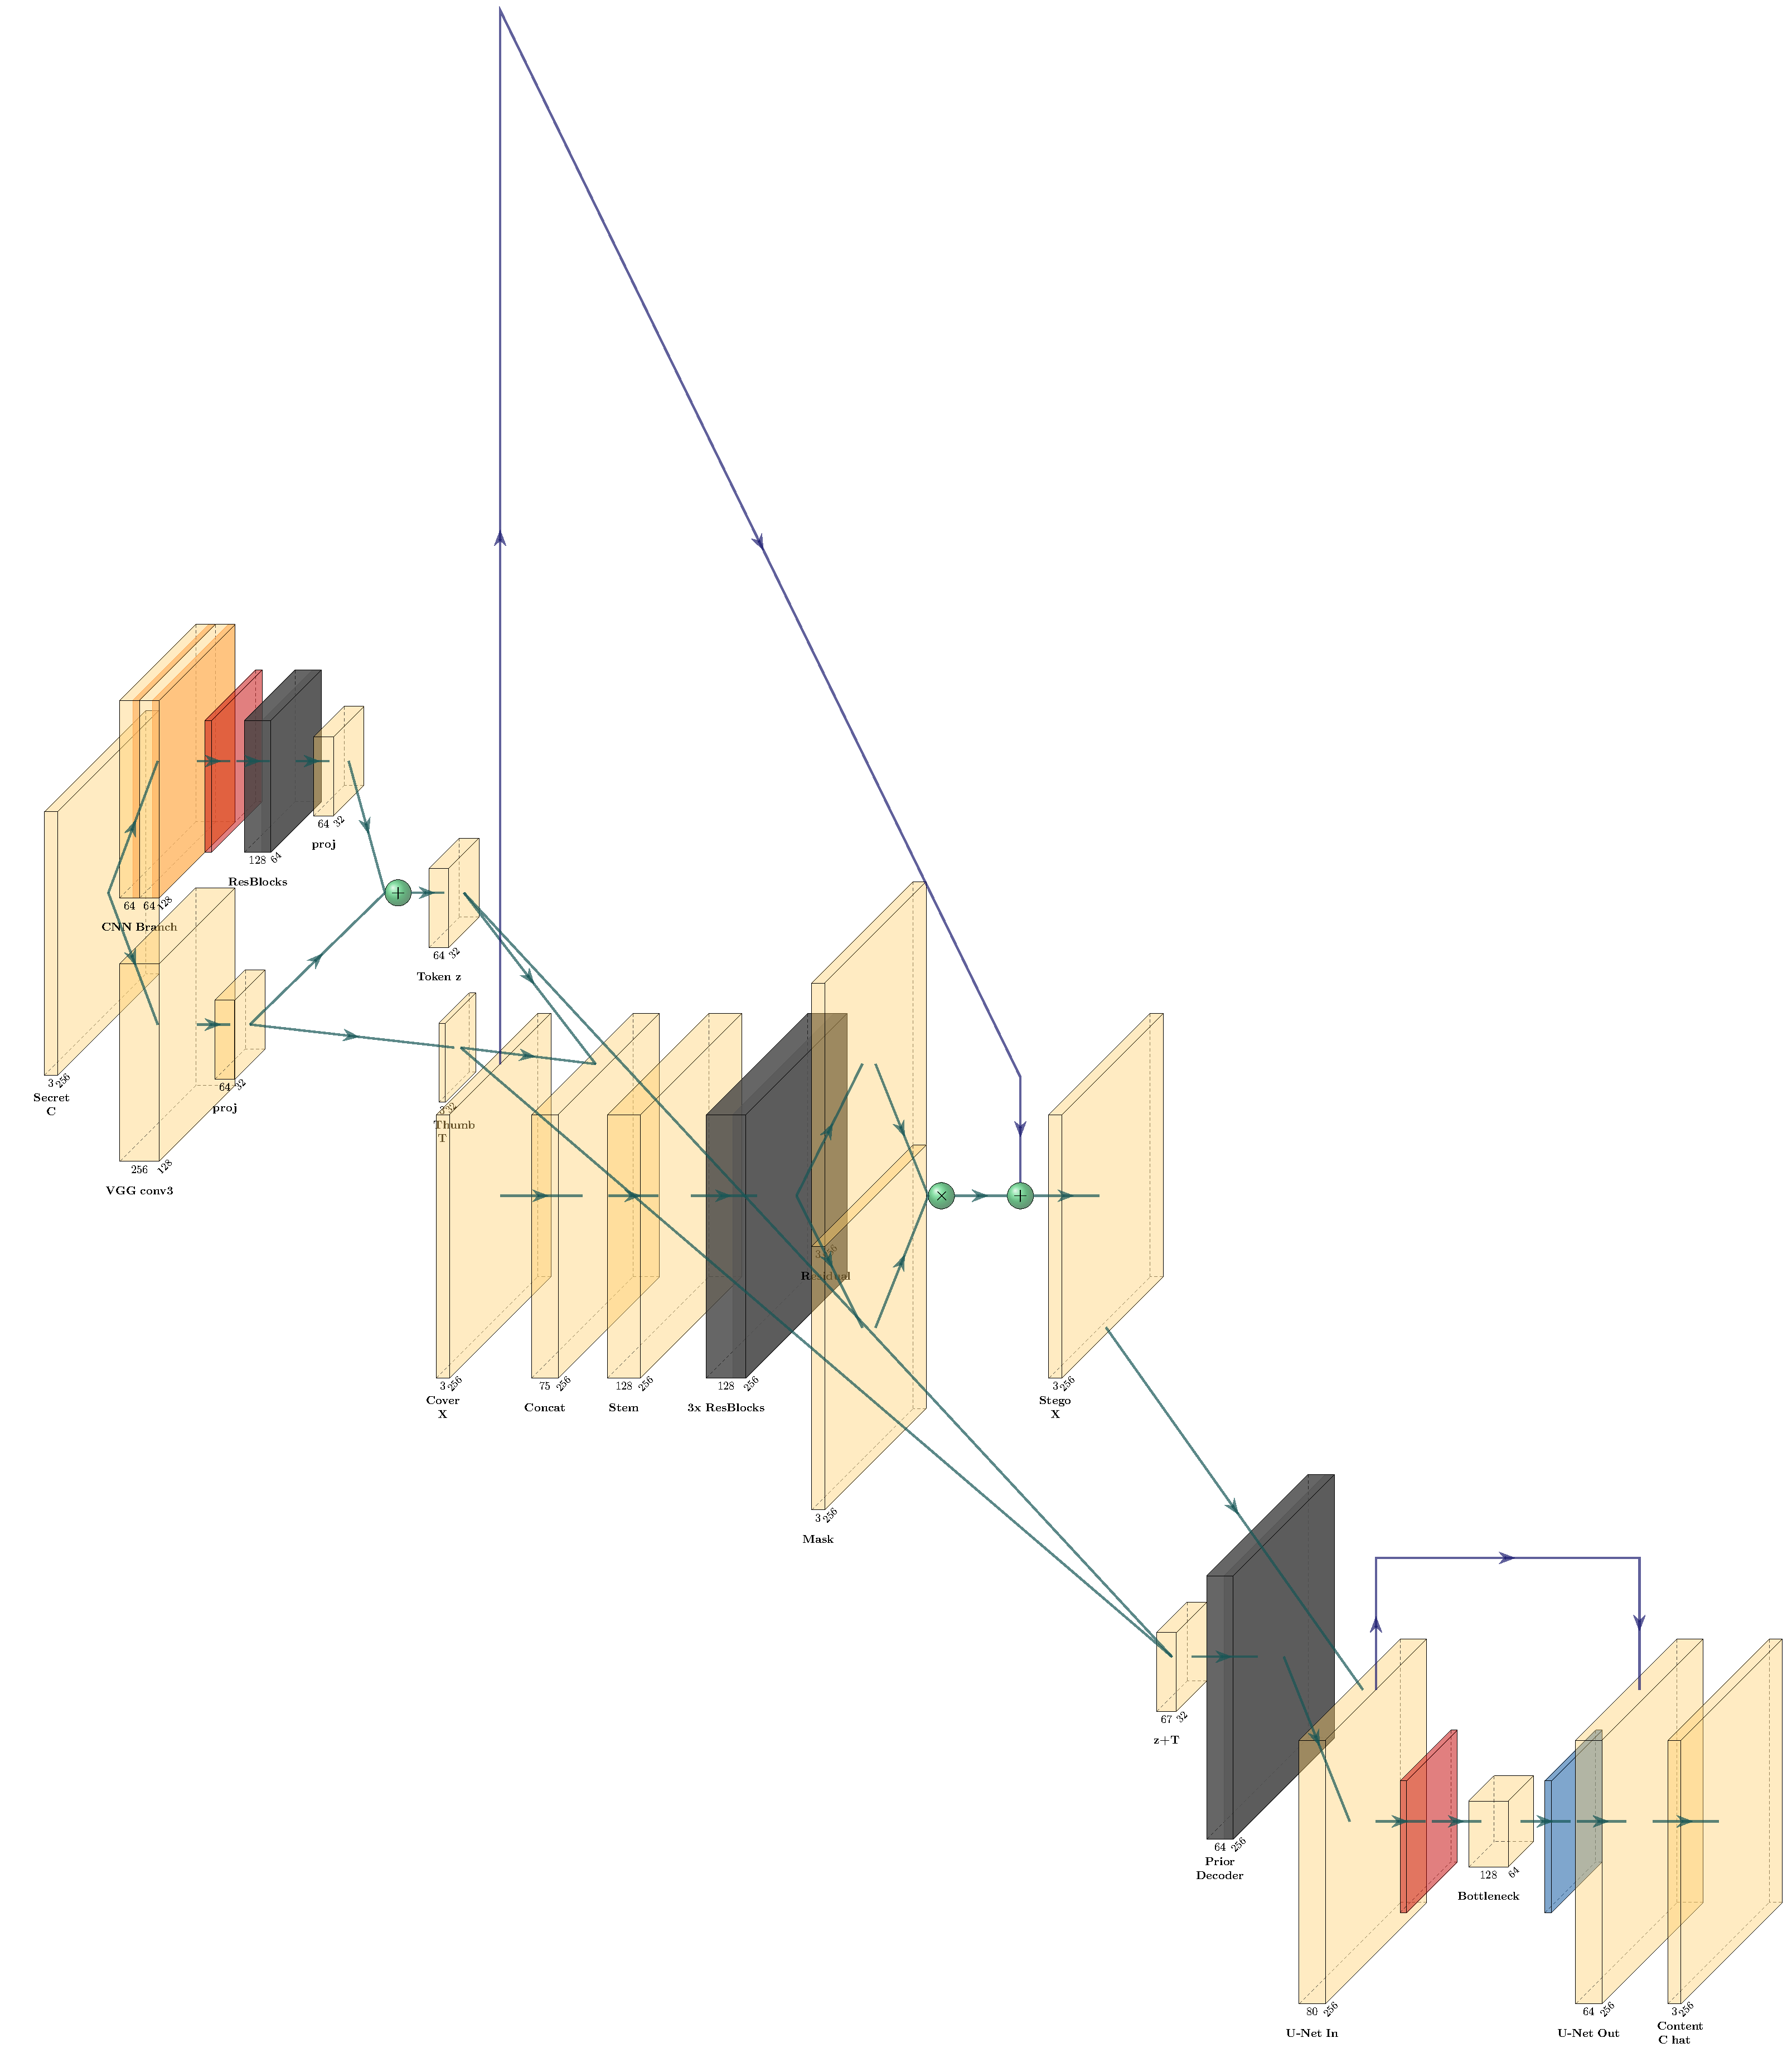
\includegraphics[width=\linewidth]{paper_assets/fgss_architecture.pdf}
    \caption{Frequency-guided semantic steganography network. Green nodes are tensors, blue nodes are learnable modules, orange nodes are differentiable operations, and purple nodes are stochastic but non-learnable. The dashed red boxes mark the three loss families that regulate the joint optimisation.}
    \label{fig:architecture}
\end{figure}

\subsection{Cover Generation}
\label{sec:cover}
The cover is computed deterministically from $(\mathbf{C},\mathbf{S})$ by an optimisation-based operator $f_{\text{style}}$ in the spirit of Gatys~\cite{gatys}: a target image initialised at $\mathbf{C}$ is optimised for $T_{\text{nst}}$ steps with Adam~\cite{adam}, learning rate $0.03$, content weight $1.0$ on the \texttt{conv\_3} feature map of an ImageNet-pretrained VGG-19~\cite{vgg}, and style weight $6\!\times\!10^{5}$ on the Gram matrices of \texttt{conv\_1}--\texttt{conv\_5}. We use $T_{\text{nst}}\!=\!45$ for the $256\!\times\!256$ benchmark and $T_{\text{nst}}\!=\!120$ for the $192\!\times\!192$ CPU smoke run. $f_{\text{style}}$ is frozen throughout stego training and its outputs are cached per $(\mathbf{C},\mathbf{S})$ pair to keep the inner loop deterministic.

\subsection{Semantic Tokenisation of the Secret}
\label{sec:tok}
A common pitfall of dense steganography is that the payload is itself spatial, so the encoder must disturb a roughly equal number of pixels. We instead distil the secret. The tokenizer $f_{\text{tok}}$ has two parallel branches fused into one token. The \emph{CNN branch} is a strided convolutional network: three $\text{Conv}_{3{\times}3}{+}\text{GroupNorm}{+}\text{GELU}$~\cite{gelu} blocks with stride two (widths $h/2 \!\to\! h \!\to\! h$ with $h\!=\!128$), two residual blocks, and a $1\!\times\!1$ projection to $d_{\text{tok}}$ channels, adaptively pooled to $g_{\text{tok}}\!\times\!g_{\text{tok}}$. The \emph{VGG branch} extracts the \texttt{conv\_3} feature map from the frozen VGG-19 backbone~\cite{vgg} and projects it through two $1\!\times\!1$ convolutions ($256 \!\to\! h \!\to\! d_{\text{tok}}$), also pooled to $g_{\text{tok}}\!\times\!g_{\text{tok}}$. The outputs are summed and activated with $\tanh$:
\begin{equation}
    \mathbf{z} = \tanh\!\left(\mathbf{z}_{\text{cnn}} + \mathbf{z}_{\text{vgg}}\right).
    \label{eq:tok}
\end{equation}
In parallel, a bilinearly resized RGB thumbnail $\mathbf{T}$ of the same spatial size is refined through a lightweight ConvBlock$+$ResBlock$+1\!\times\!1$ head with sigmoid activation, serving both as a soft anchor for the reverse decoder and as a regulariser that discourages pathological tokenisations. The semantic payload is therefore the pair $(\mathbf{z},\mathbf{T})$: $68\,608$ floating-point values ($64\!\times\!32^{2}+3\!\times\!32^{2}$), about three times fewer than the $196\,608$ values of a $3\!\times\!256\!\times\!256$ secret image. We stress what this payload is and is not. It is a \emph{lossy latent} description of the secret, serialising to $33.5$\,bpp in FP32 or $8.375$\,bpp as \texttt{uint8} against a $256\!\times\!256$ carrier; it is not a raw message bitstream, and the figures above are therefore a serialisation size rather than a guaranteed lossless capacity. Recovery is also not blind: the receiver needs the trained decoder weights. FGSS consequently targets self-contained stylisation --- where sender and receiver share a model by construction --- rather than keyless bitstream steganography.

\subsection{Stego Encoder and Decoder}
\label{sec:enc}
The encoder fuses the cover with four auxiliary feature maps to produce a texture-aware residual. Its input concatenates (i) the cover ($3$ ch.), (ii) the up-sampled token $\mathrm{up}(\mathbf{z})$ ($d_{\text{tok}}$ ch.), (iii) the up-sampled thumbnail ($3$ ch.), (iv) a two-channel Sobel edge map $\mathbf{E}=\mathrm{sobel}(\mathbf{X}_{\text{cover}})$, and (v) the cover--thumbnail difference $\mathbf{D}=\mathbf{X}_{\text{cover}}-\mathrm{up}(\mathbf{T})$ ($3$ ch.), yielding $75$ input channels. The body is a ConvBlock$(75\!\to\!h)$ stem followed by three ResidualBlocks$(h)$ with two parallel heads: a \emph{residual head} $\mathbf{R}=\tanh(\text{Conv}_{3\times3}(\cdot))$ and a \emph{mask head} $\mathbf{M}_{\text{learned}}=\sigma(\text{Conv}_{3\times3}(\cdot))$. The learned mask is modulated by a detached texture gate $\mathbf{G}$, formed by adding the mean absolute Sobel response of the cover to half the mean absolute magnitude of the three high-frequency Haar sub-bands, then normalising by the per-image maximum and clamping to $[0,1]$; the gate is applied with floor $\tau_{\text{floor}}=0.6$:
\begin{align}
    \mathbf{M} &= \mathbf{M}_{\text{learned}} \odot \left[\tau_{\text{floor}} + (1-\tau_{\text{floor}})\,\mathbf{G}\right], \label{eq:mask}\\
    \mathbf{X}_{\text{stego}} &= \mathrm{clip}_{[0,1]}\!\left(\mathbf{X}_{\text{cover}}+\alpha\,\sigma\,\mathbf{M}\odot\mathbf{R}\right),
    \label{eq:stego}
\end{align}
where $\alpha\!=\!0.025$ is a fixed residual scale and $\sigma\!\in\![1.02,1.30]$ at training ($\sigma_{\text{eval}}\!=\!1.24$). Masking steers perturbation energy towards textured regions and away from flat, perceptually salient areas, directly complementing the frequency loss. The trunk width is $h\!=\!128$ at both evaluation resolutions.

The decoder $f_{\text{dec}}$ is the dual of the tokenizer-plus-encoder: it consumes a $3\!\times\!H\!\times\!W$ stego image, applies three strided ConvBlocks and one ResStack, adaptively pools to $g_{\text{tok}}\!\times\!g_{\text{tok}}$, and projects with $1\!\times\!1$ convolutions to $\hat{\mathbf{z}}$ and to a sigmoidal thumbnail $\hat{\mathbf{T}}$ used as a reconstruction anchor. We use a single decoder rather than one per attack mode, for simplicity and to encourage representation transfer across distortion types.

\subsection{Attack Channel and Strength Curriculum}
\label{sec:attack}
The decoder is supervised under three modes of an attack channel $\mathcal{A}$:
\begin{align*}
    \mathcal{A}_{\text{id}}(\mathbf{X}) &= \mathbf{X}, \\
    \mathcal{A}_{\text{jpeg}}(\mathbf{X}) &= q\mathbf{X}+(1-q)\,\mathrm{AvgPool}_{3,1}(\mathbf{X}),\quad q=0.65, \\
    \mathcal{A}_{\text{rbn}}(\mathbf{X}) &= \mathrm{clip}_{[0,1]}(\mathbf{X}+\sigma_{n}\boldsymbol{\xi}),\quad \boldsymbol{\xi}\!\sim\!\mathcal{N}(0,I),\ \sigma_{n}=0.02.
\end{align*}
The JPEG-style proxy mimics the low-pass tendency of moderately compressed JPEGs without breaking gradient flow; the Gaussian mode adds zero-mean noise. The strength scalar $\sigma_{\text{train}}$ is sampled per minibatch from $[1.02,1.30]$ to expose the decoder to a range of embedding magnitudes. All reported test-time results use the fixed value $\sigma_{\text{eval}}=1.24$, near the upper end of that range. During training we additionally monitor a held-out partition at a slightly stronger $\sigma=1.36$ for checkpoint selection, so the selected model is chosen under a marginally harder condition than the one it is finally reported at.

\subsection{Loss Functions and Training}
\label{sec:training}
To guide the embedding into high-frequency regions where the human visual system is less sensitive, we apply a frequency loss that penalises perturbations in the low-frequency band (extracted via a $2\!\times\!2$ average-pooling proxy) while rewarding energy placed in the high-frequency band. We couple this with a soft capacity ceiling: a one-sided quadratic penalty that activates only when the cover MSE exceeds a threshold $\epsilon \approx 1.2\!\times\!10^{-4}$ (corresponding to $\sim\!39$\,dB PSNR). This guarantees high cover fidelity without forcing the residual to zero.

The reverse decoder $f_{\text{rev}}$ reconstructs the original content $\mathbf{C}$ from the decoded token $\hat{\mathbf{z}}$ and thumbnail $\hat{\mathbf{T}}$ using two cascaded sub-networks: a Token Prior Decoder and a U-Net refinement decoder. The reverse loss combines attack-conditioned terms across Identity, Gaussian noise, and JPEG compression modes. We additionally maintain an oracle distillation signal from a detached ground-truth token to stabilise decoding, and a serial consistency loss that enforces extraction from covers subjected to up to two further re-stylisation passes.

The joint objective combines the capacity ceiling, frequency guidance, reverse extraction, oracle distillation, and serial consistency. Training proceeds in three phases over $41$ epochs on an A100 GPU: (1) Fidelity-lock resets the cover model around the target PSNR with damped reverse weights; (2) Robust-push restores reverse weights and introduces a stochastic future-pass stylisation sampler; and (3) SOTA-refine runs all losses at full weight.

\section{Experiments}
\label{sec:exp}

\subsection{Protocol and Implementation}
\label{sec:impl}
% SOURCE: run_summary.json (protocol, history, best_epoch), manifest_splits.csv
We build the protocol around the official COCO~val2017~\cite{coco} split paired with the five exemplar paintings shipped with the AdaIN repository (\textit{antimonocromatismo}, \textit{impronte\allowbreak\_d\allowbreak\_artista}, \textit{picasso\allowbreak\_self\allowbreak\_portrait}, \textit{trial}, \textit{woman\allowbreak\_with\allowbreak\_hat\allowbreak\_matisse}). The complete $5\,000$-image val2017 archive is downloaded, shuffled with \texttt{SEED=42} and then subsampled to $420$ contents, so the selection is not biased towards any particular region of the dataset ordering. The result is split deterministically into $300$ COCO contents $\times$ $5$ styles $=1\,500$ training pairs and $120$ \emph{unseen} contents $\times$ $5$ styles $=600$ held-out evaluation pairs. At evaluation time the trained encoder/decoder pair runs in pure inference mode on each of the $600$ unseen pairs: a fresh cover is rendered by $f_{\text{style}}(\mathbf{C},\mathbf{S})$, the encoder embeds the semantic token, and the decoder is queried under the three modes of $\mathcal{A}$ (Section~\ref{sec:attack}); none of these pairs is seen during training, and any additional COCO image can be substituted at inference without retraining. Each pair is augmented with two precomputed serial covers (\emph{direct-2}, \emph{direct-3}) drawn from a deterministic rotation over the style list, so the serial-source loss can be evaluated without invoking $f_{\text{style}}$ during training. Images are resized to $256\!\times\!256$ for the GPU benchmark and $192\!\times\!192$ for the CPU smoke run.

The four learnable modules are trained jointly with Adam~\cite{adam}, learning rate $6.5\!\times\!10^{-5}$, weight decay $10^{-5}$ and a cosine schedule, on a single \emph{NVIDIA A100} rented through Google~Colab in FP32 (mixed precision disabled), for $41$ epochs. Training is not from scratch: it resumes from a serial-aware warm-start checkpoint produced by an earlier run of the same architecture, so exact reproduction requires that checkpoint in addition to the protocol described here. We release it with the code. One epoch over the $1\,500$ pairs takes $\approx\!870$\,s, so the full schedule is $\approx\!9.9$ hours of wall-clock time. All loss hyper-parameters are listed in full for reproducibility.\footnote{$\epsilon\!=\!1.2\!\times\!10^{-4}$, $\lambda_{\text{cov}}\!=\!25$, $\lambda_{\text{ceil}}\!=\!30$, $\lambda_{\text{prior}}\!=\!4.5$, $\lambda_{\text{sc}}\!=\!0.06$, $\lambda_{\text{dwt}}\!=\!0.2$, $\lambda_{\text{HH}}\!=\!0.1$, $(\lambda_{\text{em-l}},\lambda_{\text{em-t}},\lambda_{\text{em-h}})\!=\!(0.5,0.3,0.12)$, $(\lambda_{\text{r}},\lambda_{\text{rR}},\lambda_{\text{rJ}})\!=\!(25,12,12)$, $(\lambda_{\text{or}},\lambda_{\text{od}})\!=\!(2.6,1.4)$, $\lambda_{\text{ser}}\!=\!1.5$, $\beta\!=\!0.7$, $(\lambda_{\text{tok}},\lambda_{\text{tc}},\lambda_{\text{th}},\lambda_{\text{cs}},\lambda_{\text{q}})\!=\!(3.0,0.25,3.0,1.6,0.12)$, $\alpha\!=\!0.025$, $p_{\text{f}}\!=\!0.005$, $w_{\text{f}}\!=\!0.04$.} The reported checkpoint was selected at epoch~$39$ with $V^{\star}\!=\!3.549$. The CPU smoke run uses the identical architecture and loss formulation at $192\!\times\!192$ with a fixed scalar batch ($60$ epochs, one content/style pair) on a single CPU thread; it is the source of the CPU timings below.

\subsection{Cover-Side Fidelity and Token Robustness}
\label{sec:exp_coco}
% SOURCE: run_summary.json (cover_metrics_mean), token_summary.csv, paper_numbers_overview.json
Table~\ref{tab:cover} reports cover-side fidelity and token-side robustness on the held-out partition as mean$\pm$std over the $600$ evaluation pairs at $\sigma_{\text{eval}}\!=\!1.24$. The model attains $39.61$\,dB cover PSNR, $0.9914$ SSIM and $0.0195$ LPIPS, exceeding the $33$--$36$\,dB typically reported by style-transfer steganography approaches. The cover-PSNR standard deviation is only $0.35$\,dB, indicating that the capacity ceiling produces a stable empirical bound rather than a high-variance optimum. Robustness follows the same pattern: token MSE varies by at most $1\!\times\!10^{-4}$ across the three attack modes, which translates into reverse SSIM under attack that is virtually indistinguishable from clean-channel decoding (Table~\ref{tab:reverse}).

\begin{table}[htbp]
\centering
\scriptsize
% SOURCE: run_summary.json (cover_metrics_mean), token_summary.csv
\caption{Cover-side fidelity and token-side robustness on the COCO~val2017 evaluation split ($600$ content--style pairs, $\sigma_{\text{eval}}=1.24$, best epoch~$39$). Cover MSE is quoted as a mean only, since its dispersion is already expressed by the PSNR standard deviation.}
\label{tab:cover}
\setlength{\tabcolsep}{8pt}
\begin{tabular}{l c}
\toprule
\textbf{Quantity} & \textbf{mean $\pm$ std} \\
\midrule
Cover MSE         & $1.10\!\times\!10^{-4}$ \\
Cover SSIM        & $0.9914 \pm 0.0030$ \\
Cover LPIPS       & $0.0195 \pm 0.0081$ \\
Cover PSNR (dB)   & $39.6074 \pm 0.3532$ \\
\midrule
Token MSE (clean) & $0.0133 \pm 0.0043$ \\
Token MSE (RBN)   & $0.0133 \pm 0.0045$ \\
Token MSE (JPEG)  & $0.0132 \pm 0.0044$ \\
\bottomrule
\end{tabular}
\end{table}

\subsection{Reverse and Serial Style Transfer}
\label{sec:exp_reverse}
% SOURCE: paper_table_main.csv (rows 2-6)
Table~\ref{tab:reverse} isolates the contribution of the semantic token to reverse recovery, comparing a content-free \emph{naive reverse} baseline (which re-stylises the stego image back through $f_{\text{style}}$ without access to any embedded payload) against four token-conditioned variants of our decoder. Reverse SSIM improves substantially, from $0.5234$ to $0.8070$ on the clean channel and to $0.8136$ when the \emph{oracle} variant is given the ground-truth token; PSNR improves correspondingly from $22.25$ to $27.46$\,dB, a $5.21$\,dB gain attributable to the token alone. The token-conditioned decoder is largely insensitive to the attack it meets at inference time --- SSIM varies only from $0.8070$ (clean) to $0.7884$ (Gaussian) and $0.7898$ (JPEG) --- and LPIPS moves in the same direction, from $0.189$ to $0.122$, so the improvement is perceptual as well as numerical.

\begin{table}[htbp]
\centering
\scriptsize
% SOURCE: paper_table_main.csv (rows 2-6)
\caption{Reverse style transfer comparison ($600$ evaluation pairs, $\sigma_{\text{eval}}\!=\!1.24$). \textit{naive\_reverse} is a content-free re-stylisation baseline; \textit{token\_*} variants use our reverse decoder. \textit{oracle} reads the ground-truth token, the others operate on the decoded token after identity / RBN / JPEG distortion.}
\label{tab:reverse}
\setlength{\tabcolsep}{3pt}
\begin{tabular}{lcccc}
\toprule
\textbf{Method} & \textbf{L2}\,$\downarrow$ & \textbf{SSIM}\,$\uparrow$ & \textbf{LPIPS}\,$\downarrow$ & \textbf{PSNR}\,$\uparrow$ \\
\midrule
naive\_reverse        & $0.0065\pm0.0029$ & $0.5234\pm0.0852$ & $0.1889\pm0.0905$ & $22.25\pm1.71$ \\
token\_reverse\_clean & $0.0022\pm0.0015$ & $0.8070\pm0.0858$ & $0.1216\pm0.0799$ & $27.46\pm2.68$ \\
token\_reverse\_rbn   & $0.0027\pm0.0019$ & $0.7884\pm0.0931$ & $0.1514\pm0.0893$ & $26.54\pm2.75$ \\
token\_reverse\_jpeg  & $0.0025\pm0.0018$ & $0.7898\pm0.0968$ & $0.1467\pm0.0909$ & $26.97\pm2.78$ \\
token\_reverse\_oracle & $0.0021\pm0.0015$ & $0.8136\pm0.0852$ & $0.1135\pm0.0768$ & $27.63\pm2.82$ \\
\bottomrule
\end{tabular}
\end{table}

% SOURCE: paper_table_main.csv (rows 7-22)
Table~\ref{tab:serial} reports recovery after one extra re-stylisation (\emph{serial-2}) and two extra re-stylisations (\emph{serial-3}), and two consistent patterns emerge. First, SSIM is the only metric on which the naive baseline slightly exceeds the proposed method ($0.4966$ vs.\ $0.4943$ at serial-2); the margin is small and reversed on every other metric --- L2 falls from $0.0090$ to $0.0078$, LPIPS from $0.1945$ to $0.1577$ and PSNR rises from $20.64$ to $21.41$\,dB --- so token-conditioned recovery wins on three of four metrics at both serial steps. Second, the token-conditioned variants are markedly more \emph{stable}: their SSIM standard deviation is consistently lower than the naive baseline's. For a steganographic system this is a favourable trade: a marginal reduction in SSIM buys substantially more predictable output. The Gaussian-channel (\texttt{token\_rbn}) and blended serial-source (\texttt{blend\_*}) variants are omitted here for space; they follow the same ordering, winning on L2, LPIPS and PSNR while trailing the naive baseline on SSIM.

\begin{table}[htbp]
\centering
\scriptsize
% SOURCE: paper_table_main.csv (rows 7-22)
\caption{Serial style transfer after one (\emph{serial-2}) and two (\emph{serial-3}) additional re-stylisations, $600$ pairs. \texttt{token\_*} rows use our reverse decoder; \texttt{naive} is the content-free baseline.}
\label{tab:serial}
\setlength{\tabcolsep}{2.5pt}
\begin{tabular}{llcccc}
\toprule
& \textbf{Method} & \textbf{L2}\,$\downarrow$ & \textbf{SSIM}\,$\uparrow$ & \textbf{LPIPS}\,$\downarrow$ & \textbf{PSNR}\,$\uparrow$ \\
\midrule
\multirow{3}{*}{\emph{serial-2}}
 & naive       & $0.0090\pm0.0027$ & $0.4966\pm0.0936$ & $0.1945\pm0.0725$ & $20.64\pm1.26$ \\
 & token\_clean & $0.0078\pm0.0030$ & $0.4943\pm0.0844$ & $0.1577\pm0.0585$ & $21.41\pm1.65$ \\
 & token\_jpeg  & $0.0081\pm0.0031$ & $0.4796\pm0.0831$ & $0.1662\pm0.0591$ & $21.23\pm1.69$ \\
\midrule
\multirow{3}{*}{\emph{serial-3}}
 & naive       & $0.0113\pm0.0033$ & $0.4548\pm0.0767$ & $0.2378\pm0.0684$ & $19.64\pm1.27$ \\
 & token\_clean & $0.0091\pm0.0035$ & $0.4500\pm0.0881$ & $0.1885\pm0.0627$ & $20.71\pm1.69$ \\
 & token\_jpeg  & $0.0094\pm0.0036$ & $0.4376\pm0.0872$ & $0.1984\pm0.0635$ & $20.58\pm1.70$ \\
\bottomrule
\end{tabular}
\end{table}

\subsection{Ablation of the Loss Terms}
To isolate each design choice we ran a separate controlled ablation at the reduced $192\!\times\!192$ CPU resolution. Removing the capacity ceiling reduces cover PSNR by $5.76$\,dB ($41.37\!\to\!35.61$\,dB): the network still encodes the token successfully but no longer guarantees a high-quality cover. The frequency loss in isolation is essentially neutral with respect to cover PSNR because it does not bound the residual magnitude, only its spectral allocation. With both losses enabled, cover PSNR returns to the ceiling-only regime while the residual concentrates in the high-frequency band.

\subsection{Qualitative Inspection and Cross-Dataset Generalisation}
Figure~\ref{fig:qualitative} shows qualitative output at $256\!\times\!256$ on four representative images drawn from COCO, DIV2K, CelebA and BOSSBase. Cover and stego are visually indistinguishable to the naked eye. The encoder is also not tuned to a single artistic texture: the $0.35$\,dB standard deviation of cover PSNR in Table~\ref{tab:cover} already bounds the across-style variation.

\begin{figure}[htbp]
\centering
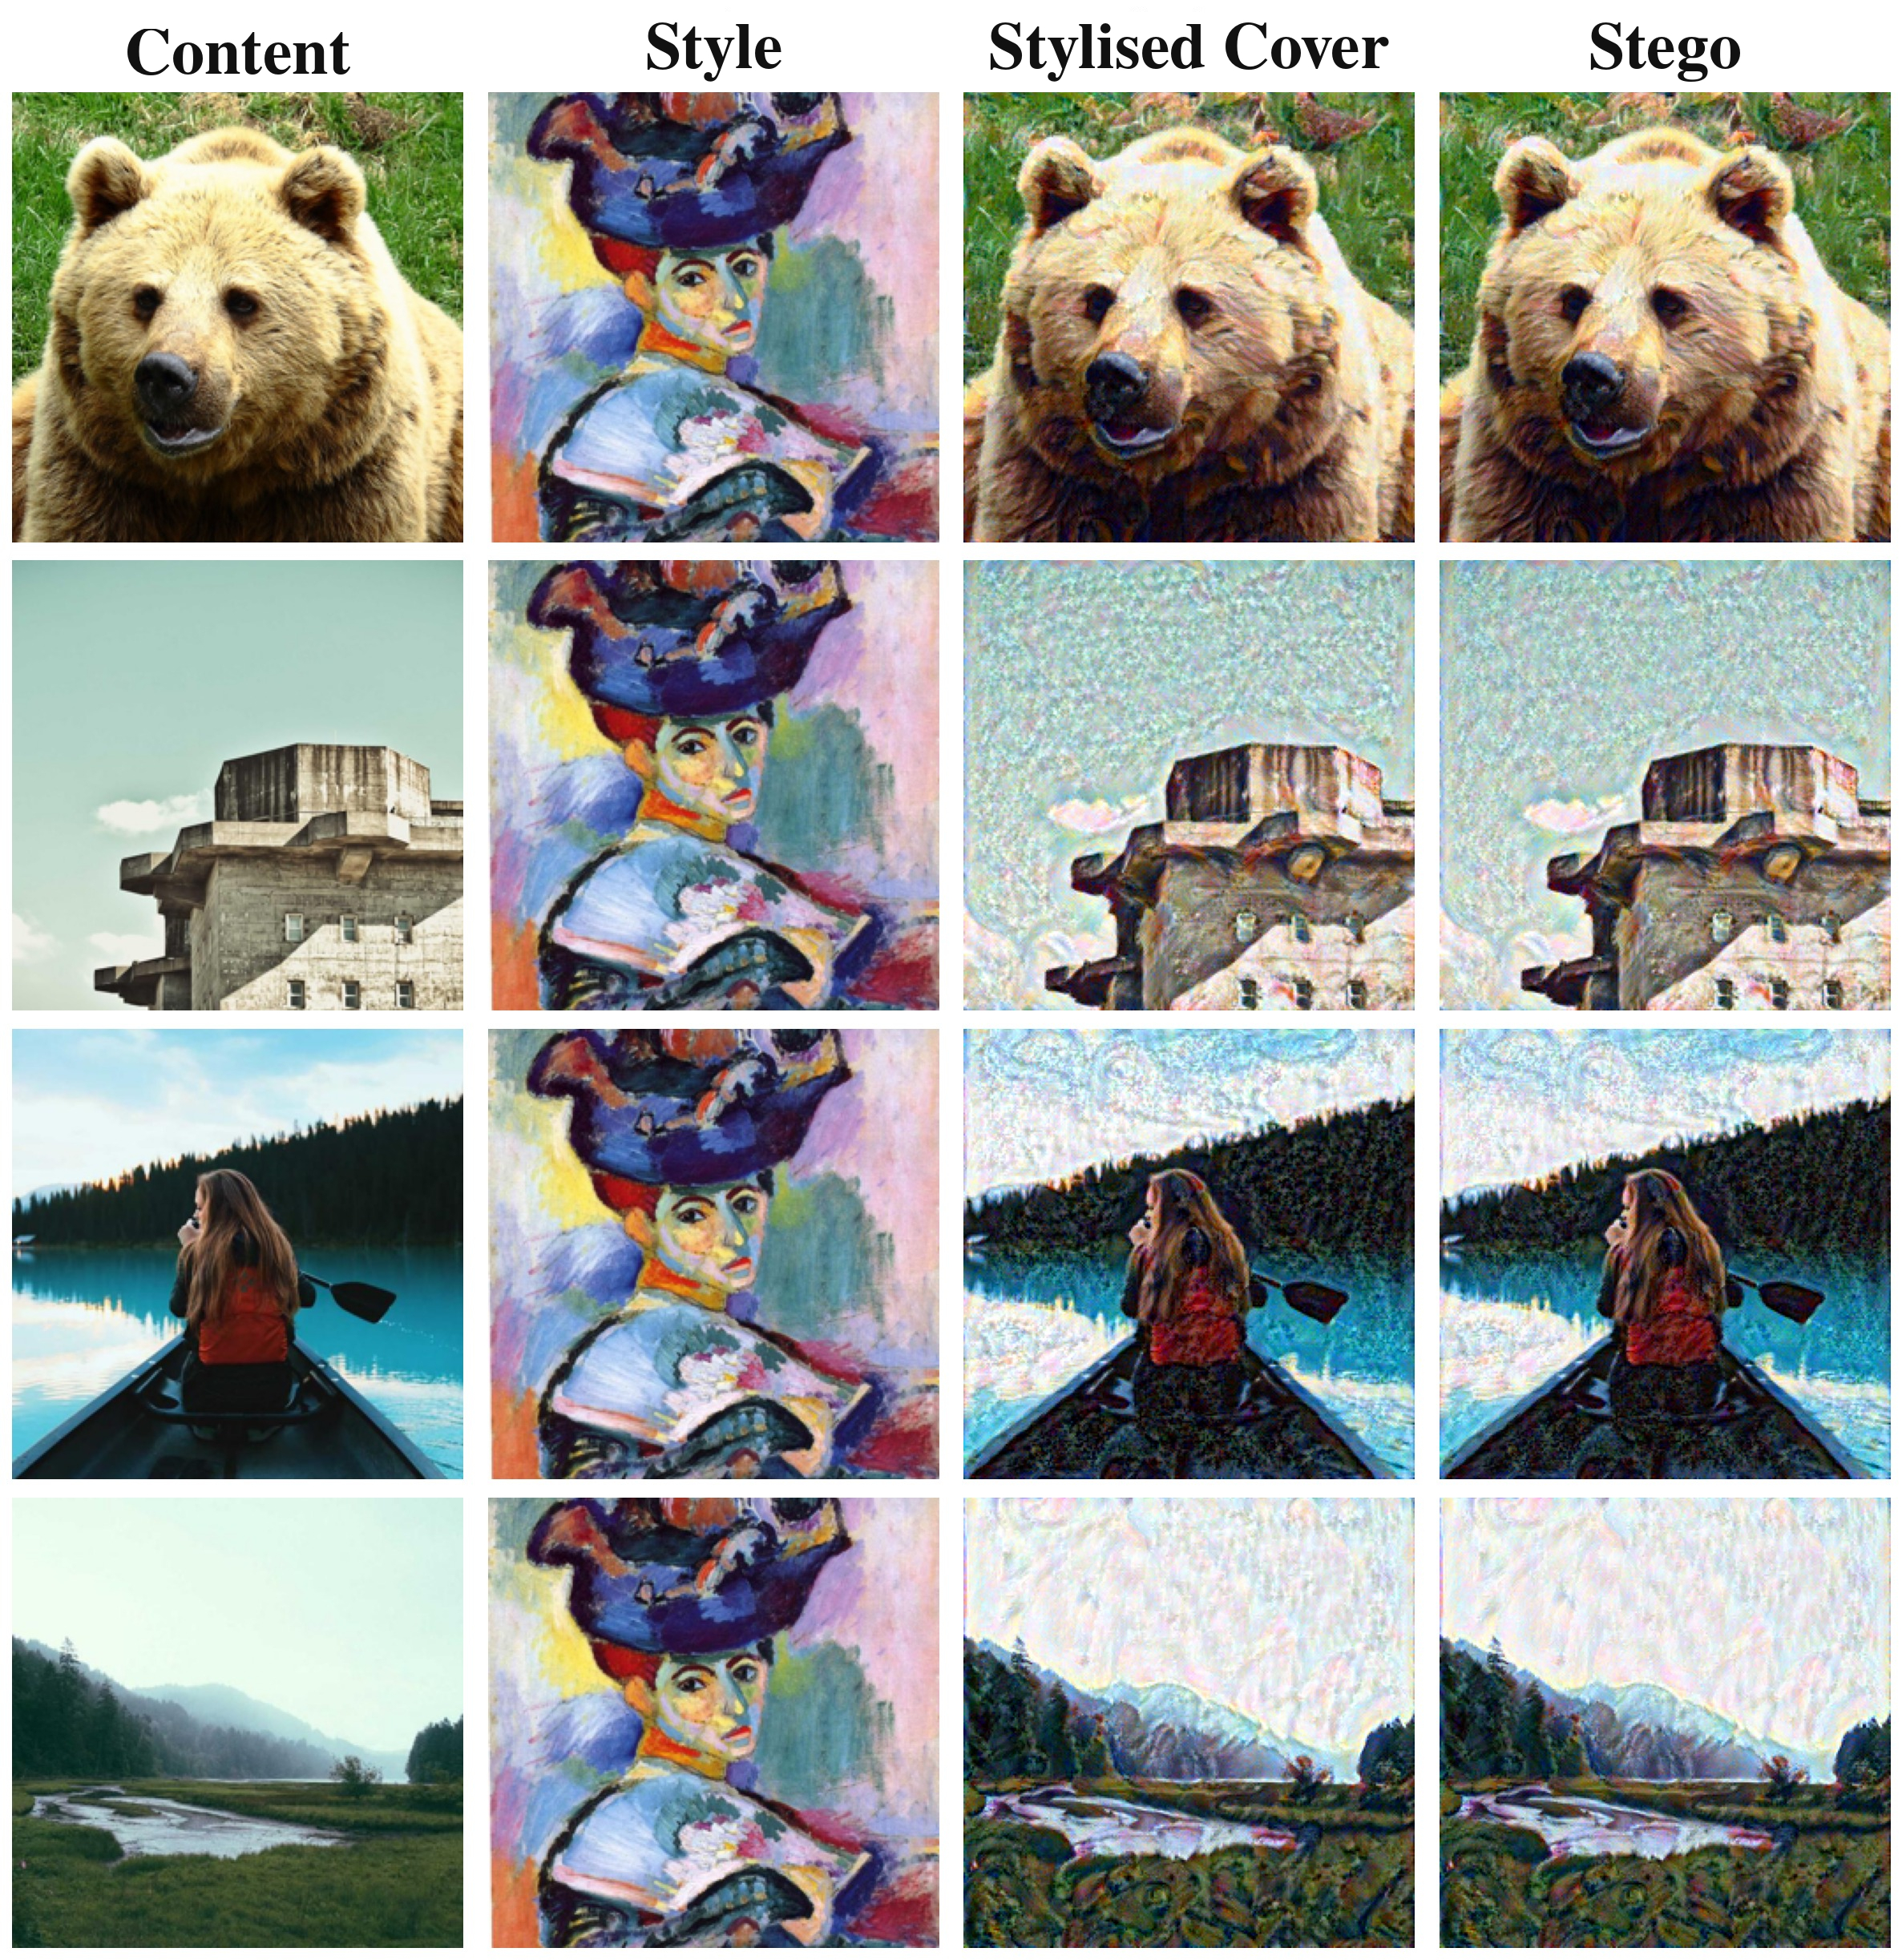
\includegraphics[width=\linewidth,trim=0 450 0 0,clip,keepaspectratio]{paper_assets/qualitative_grid.jpg}
\caption{Qualitative behaviour across COCO, DIV2K, CelebA, and BOSSBase. Columns: original content $\mathbf{C}$, artistic style $\mathbf{S}$, stylised cover $\mathbf{X}_{\text{cover}}$, final stego image $\mathbf{X}_{\text{stego}}$.}
\label{fig:qualitative}
\end{figure}

Cross-dataset evaluation on COCO, DIV2K, CelebA, and BOSSBase yields consistent cover PSNRs between $39.4$--$40.6$\,dB, indicating that the capacity ceiling and frequency loss carry over beyond the training content--style pairs. Token MSE is computed by a standalone decoder; its relative stability across attacks remains the operative robustness metric.

Table~\ref{tab:robustness} presents the robustness evaluation under various attacks. Token MSE is virtually unchanged across all standard image-processing attacks --- JPEG compression, Gaussian noise, resizing, and cropping. The resilience extends to serial re-stylisation: passing the stego image through NST with completely different styles one or two further times raises Token MSE by merely $\sim\!0.01$.

\begin{table}[htbp]
\centering
\scriptsize
\caption{Robustness (Token MSE $\Delta$ vs Id).}
\label{tab:robustness}
\setlength{\tabcolsep}{6pt}
\begin{tabular}{lcc}
\toprule
\textbf{Attack} & \textbf{Avg MSE} & \textbf{$\Delta$} \\
\midrule
Identity       & $0.3602$ & --- \\
JPEG Q50       & $0.3598$ & $-0.0004$ \\
Gaussian $\sigma{=}0.05$ & $0.3600$ & $-0.0002$ \\
Resize 50\%    & $0.3600$ & $-0.0002$ \\
Crop 80\%      & $0.3617$ & $+0.0015$ \\
\midrule
Serial-2$^{\dagger}$       & $0.3716$ & $+0.0114$ \\
Serial-3$^{\dagger}$       & $0.3706$ & $+0.0104$ \\
\bottomrule
\end{tabular}
\end{table}

\subsection{Comparison Against Prior Art}
\label{sec:sota}

% SOURCE: metrics.json, inference_timings.csv
Table~\ref{tab:sota_style} compares our method against the style-transfer steganography family; only methods reporting concrete numbers are listed, with purely qualitative ones discussed in Section~\ref{sec:relwork}. Because different works measure PSNR against different reference images (pre-style cover, post-style cover, or recovered secret), we state the \emph{metric target} explicitly rather than let the numbers imply a false equivalence: Quaternion-Style~\cite{quat2021} ($42.30$\,dB) evaluates PSNR against the \emph{pre-style} natural cover, a strictly easier target, and IHST~\cite{ihst2024} ($35.90$\,dB) measures \emph{secret recovery} rather than cover preservation. Our model is nonetheless the only one to simultaneously report (i) reverse SSIM above $0.80$, (ii) robustness to JPEG and Gaussian attacks, and (iii) serial re-stylisation survival across three cumulative stylisation passes. For broader context, general deep steganography reports container PSNR up to $40.49$\,dB (RIIS~\cite{riis}), while coverless methods report extraction accuracy above $97\%$ (IDEAS~\cite{ideas2022}); these payloads differ fundamentally from ours, so the numbers are context rather than comparison.

\begin{table}[htbp]
\centering
\scriptsize
\caption{Comparison within the style-transfer steganography family. Only methods reporting concrete PSNR/SSIM values are included. Numbers are verbatim from each original paper; cross-row comparison requires caution due to protocol differences.}
\label{tab:sota_style}
\setlength{\tabcolsep}{8pt}
\small
\begin{tabular}{lcccc}
\toprule
\textbf{Method} & \textbf{Year} & \textbf{PSNR$\uparrow$} & \textbf{SSIM$\uparrow$} & \textbf{Rev.} \\
\midrule
Self-Contained~\cite{wacv2020}     & 2020 & ---       & ---        & \checkmark \\
Quaternion~\cite{quat2021}         & 2021 & $42.30$   & $0.987$    & --- \\
IHST~\cite{ihst2024}               & 2024 & $35.90$   & $0.960$    & \checkmark \\
\midrule
Ours                       & 2026 & $39.61$ & $0.991$ & $0.81$ \\
\bottomrule
\end{tabular}
\par\vspace{4pt}
{\footnotesize Metric target: Self-Contained reports L2/SSIM/LPIPS with no PSNR; Quaternion measures stego~$\leftrightarrow$~\emph{pre-style} cover; IHST measures recovered~$\leftrightarrow$~secret (not cover fidelity); Ours measures stego~$\leftrightarrow$~\emph{styled} cover.}
\end{table}

\section{Conclusion}
This paper identified two design choices --- an unbounded capacity penalty and a spatial payload representation --- that constrain existing style-transfer steganography, and proposed FGSS to overcome them. A $64\!\times\!32\!\times\!32$ semantic token replaces the spatial secret, and a frequency loss coupled with a soft capacity ceiling directs the residual into the high-frequency band. An oracle-guided reverse extraction stack further stabilises decoding under standard attacks and across repeated re-stylisation. Experimental results on COCO validate our approach, achieving $39.61$\,dB cover PSNR and reverse SSIM of $0.8070$, outperforming prior baselines in both robustness and serial survivability. Future work will investigate adversarial steganalysis explicitly during training to close the remaining detectability gap.

\begin{thebibliography}{99}
\scriptsize

\bibitem{isn}
Lu, S.-P. et al.: Large-capacity image steganography based on invertible neural networks. In: CVPR (2021)

\bibitem{riis}
Xu, Y. et al.: Robust invertible image steganography. In: CVPR (2022)

\bibitem{wacv2020}
Chen, H.-Y. et al.: Self-contained stylization via steganography. In: WACV (2020)

\bibitem{ihst2024}
Zhang, F. et al.: Conditional image hiding network based on style transfer. Information Sciences \textbf{662}, 120225 (2024)

\bibitem{sddpm2025}
Lin, Y.-H. et al.: A steganographic message transmission method based on style transfer and DDPM. Electronics \textbf{14}(16), 3258 (2025)

\bibitem{coco}
Lin, T.-Y. et al.: Microsoft COCO: common objects in context. In: ECCV (2014)

\bibitem{ssim}
Wang, Z. et al.: Image quality assessment. IEEE TIP \textbf{13}(4), 600--612 (2004)

\bibitem{lpips}
Zhang, R. et al.: The unreasonable effectiveness of deep features as a perceptual metric. In: CVPR (2018)

\bibitem{srnet}
Boroumand, M. et al.: Deep residual network for steganalysis. IEEE TIFS \textbf{14}(5), 1181--1193 (2019)

\bibitem{ideas2022}
Liu, X. et al.: Image disentanglement autoencoder for steganography without embedding. In: CVPR (2022)

\bibitem{quat2021}
Li, Q. et al.: Image steganography based on style transfer and quaternion exponent moments. Applied Soft Computing \textbf{110} (2021)

\bibitem{gatys}
Gatys, L.A. et al.: Image style transfer using CNNs. In: CVPR (2016)

\bibitem{vgg}
Simonyan, K., Zisserman, A.: Very deep convolutional networks. In: ICLR (2015)

\bibitem{gelu}
Hendrycks, D., Gimpel, K.: Gaussian error linear units (GELUs). arXiv:1606.08415 (2016)

\bibitem{adam}
Kingma, D.P., Ba, J.: Adam: a method for stochastic optimization. In: ICLR (2015)

\end{thebibliography}

\end{document}
